% Compact PGFPlots panel for the surface5 bit-scale decomposition.
% Requires \usepackage{pgfplots} and \pgfplotsset{compat=1.18}.
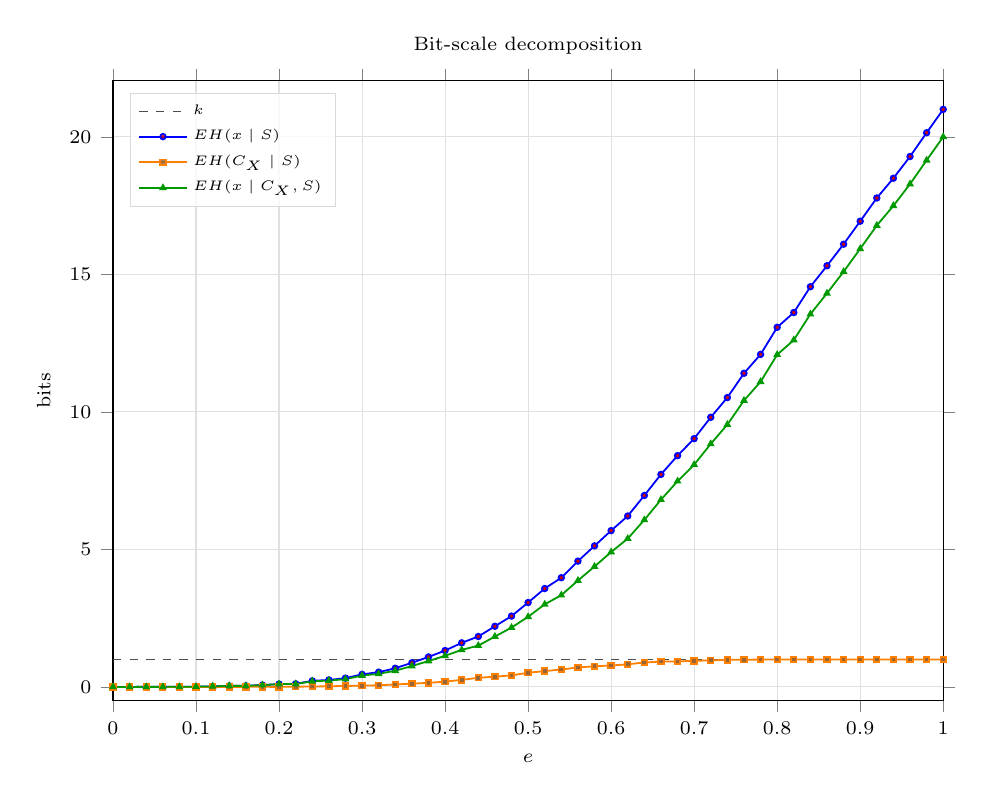
\begin{tikzpicture}
\begin{axis}[
  name=surfaceFiveBitScaleAxis,
  width=\linewidth,
  height=0.78\linewidth,
  title={Bit-scale decomposition},
  title style={font=\scriptsize},
  xlabel={$e$},
  ylabel={bits},
  xmin=0, xmax=1,
  ymin=-0.5, ymax=22.05,
  grid=both,
  major grid style={black!12},
  minor grid style={black!6},
  tick align=outside,
  tick label style={font=\scriptsize},
  label style={font=\scriptsize},
  legend cell align={left},
  legend style={draw=black!15, fill=white, fill opacity=0.82, text opacity=1, at={(0.02,0.98)}, anchor=north west, font=\tiny},
]
\addplot[black!70, dashed, line width=0.55pt] coordinates {(0,1) (1,1)};
\addlegendentry{$k$}
\addplot+[color=blue, mark=*, mark size=1.0pt, line width=0.65pt]
coordinates {(0,0) (0.02,0) (0.04,0.002) (0.06,0.002) (0.08,0.005) (0.1,0.008) (0.12,0.022) (0.14,0.037) (0.16,0.041) (0.18,0.068) (0.2,0.104) (0.22,0.113) (0.24,0.221) (0.26,0.253) (0.28,0.319) (0.3,0.457) (0.32,0.537) (0.34,0.679) (0.36,0.878) (0.38,1.09) (0.4,1.323) (0.42,1.603) (0.44,1.833) (0.46,2.204) (0.48,2.575) (0.5,3.068) (0.52,3.577) (0.54,3.971) (0.56,4.574) (0.58,5.129) (0.6,5.683) (0.62,6.215) (0.64,6.962) (0.66,7.727) (0.68,8.408) (0.7,9.028) (0.72,9.804) (0.74,10.522) (0.76,11.404) (0.78,12.09) (0.8,13.076) (0.82,13.613) (0.84,14.551) (0.86,15.313) (0.88,16.098) (0.9,16.933) (0.92,17.778) (0.94,18.496) (0.96,19.285) (0.98,20.15) (1,21)};
\addlegendentry{$\mathbb{E}H(x\mid S)$}
\addplot+[color=orange, mark=square*, mark size=1.0pt, line width=0.65pt]
coordinates {(0,0) (0.02,0) (0.04,0) (0.06,0) (0.08,0) (0.1,0) (0.12,0.001) (0.14,0) (0.16,0.003) (0.18,0.003) (0.2,0.002) (0.22,0.007) (0.24,0.016) (0.26,0.023) (0.28,0.036) (0.3,0.044) (0.32,0.061) (0.34,0.09) (0.36,0.119) (0.38,0.148) (0.4,0.192) (0.42,0.256) (0.44,0.332) (0.46,0.372) (0.48,0.418) (0.5,0.517) (0.52,0.574) (0.54,0.634) (0.56,0.706) (0.58,0.751) (0.6,0.779) (0.62,0.822) (0.64,0.889) (0.66,0.92) (0.68,0.928) (0.7,0.947) (0.72,0.967) (0.74,0.983) (0.76,0.99) (0.78,0.993) (0.8,0.996) (0.82,1) (0.84,0.997) (0.86,1) (0.88,1) (0.9,1) (0.92,1) (0.94,1) (0.96,1) (0.98,1) (1,1)};
\addlegendentry{$\mathbb{E}H(C_X\mid S)$}
\addplot+[color=green!60!black, mark=triangle*, mark size=1.0pt, line width=0.65pt]
coordinates {(0,0) (0.02,0) (0.04,0.002) (0.06,0.002) (0.08,0.005) (0.1,0.008) (0.12,0.021) (0.14,0.037) (0.16,0.038) (0.18,0.065) (0.2,0.102) (0.22,0.106) (0.24,0.205) (0.26,0.23) (0.28,0.283) (0.3,0.413) (0.32,0.476) (0.34,0.589) (0.36,0.759) (0.38,0.942) (0.4,1.131) (0.42,1.347) (0.44,1.501) (0.46,1.832) (0.48,2.157) (0.5,2.551) (0.52,3.003) (0.54,3.337) (0.56,3.868) (0.58,4.378) (0.6,4.904) (0.62,5.393) (0.64,6.073) (0.66,6.807) (0.68,7.48) (0.7,8.081) (0.72,8.837) (0.74,9.539) (0.76,10.414) (0.78,11.097) (0.8,12.08) (0.82,12.613) (0.84,13.554) (0.86,14.313) (0.88,15.098) (0.9,15.933) (0.92,16.778) (0.94,17.496) (0.96,18.285) (0.98,19.15) (1,20)};
\addlegendentry{$\mathbb{E}H(x\mid C_X,S)$}
\end{axis}
\end{tikzpicture}
